\subsection{Generative Models}
We are concerned with learning generative models that describe transformations of a source-language sequence $\ve$ to a target-language sequence $\vf$.
We consider two different settings for these models.

In the parallel data setting, both $\vx = (\ve, \vf)$ are observed. 
The generative story assigns the following probability to the event that $\vf$ arises from $\ve$:
\begin{equation}
p(\vx; \Theta) = p(\vf \mid \ve) = \sum_\va p(\va,\,\vf \mid \ve)
\label{eqn:parallel}
\end{equation}
where $\Theta$ denotes the model parameters and $\va$ denotes a hidden variable that corresponds to unknown choices taken of the generative process.
%(in our case, $\va$ is an alignment, see next subsection).

In the decipherment setting, only the target entity $\vf$ is observed and the source entity $\ve$ is considered hidden. 
Letting $\vx = (\vf)$ the decipherment model takes the form:
\begin{equation}
p(\vx; \Theta) = p(\vf) = \sum_{\ve} p(\ve) \sum_{\va} p(\va,\,\vf \mid \ve)
\label{eqn:decipherment}
\end{equation}
That is, according to the decipherment generative story, the observed entity $\vf$ can arise from any source entity $\ve$ by first selecting $\ve \sim p(\ve)$ and then proceeding according to the parallel data generative story.

Training these models entails the same objective - maximizing the observed data log-likelihood $L(\Theta \mid X)$:
\begin{align*}
\max_{\Theta}\,\,L(\Theta \mid X)
%=&\max_{\Theta}\,\,\log\prod_{n}p (\vx_n;\Theta)\\
=&\max_{\Theta}\,\,\sum_{n}\log p (\vx_n;\Theta)
\end{align*}
%_{n=1}^{N}
where $X=\set{(\ve_{n},\, \vf_{n})}_n$ in the parallel data setting and $X=\set{(\vf_{n})}_n$ in the decipherment setting.

Next, we make these generative stories concrete by explicitly defining $p(\va, \vf \mid \ve)$ and $p(\ve)$ (if necessary) in two sequence alignment tasks - word alignment and back-transliteration decipherment.

%We make the discussion concrete by discussing two related tasks - word alignment and back-transliteration. 

%The predominant approach for training these generative models 

\subsection{Parallel Data: Word Alignment}

%Keeping the discussion abstract, we consider the general problem of sequence alignment. 
%In sequence alignment, we are given a sequence $e = (e_1, \ldots, e_I)$ comprising of source language entities and a sequence $f = (f_1, \ldots, f_J)$ comprising of target language entities (concretely, these entities can represent words or phonemes in each language) and are tasked with finding an alignment 

Word alignment is one of the major building blocks in the conventional machine translation pipeline.
In word alignment, the entity $\ve = (\ve_1, \ldots, \ve_I)$ represents a sentence in the source language and $\vf = (\vf_1, \ldots, \vf_J)$ represents a sentence in the target language. 
The generative story for the transformation of $\ve$ to $\vf$ follows according to \eqn{eqn:parallel} where the hidden variable $\va = (\va_1, \ldots, \va_J)$ corresponds to a sequence of $J$ indices and encodes an asymmetric \emph{target-to-source} alignment under which the $j$th target word is aligned to the $\va_j$th source word. 
In other words, under the generative story, $\vf_j$ is thought to be generated from $\ve_{\va_j}$.

The HMM word alignment model is considered both computationally efficient and effective. However, since its objective is not convex, it is common practice to initialize training using the simpler IBM 1 model.
Both models assign the following conditional probability for a target sequence $\vf$ given an observed source sequence $\ve$ and a fixed alignment $\va$:
\begin{equation}
p(\va, \vf \mid \ve) = \prod_{j=1}^{J} t(\vf_j \mid \ve_{\va_j})\cdot a(\va_j \mid \va_{j'})
\label{eqn:WA}
\end{equation}
That is, both models are parameterized using two tables of conditional probability distributions $\Theta=(t, a)$. 
The translation table $t(\vf_j \mid \ve_{\va_j})$ encodes the probability of translating $\ve_{\va_j}$ to $\vf_j$ and the distortion table $a$ is a model dependent probability table that quantifies the probability of aligning the $j$th target position with the $\va_j$th source position, possibly given a previous alignment decision.

Specifically, IBM model 1 uses a degenerate distortion table that assigns a uniform probability to all possible source positions and the HMM model encodes distortions using a first-order dependency on the previously non null-aligned position $\va_{j'}$.
The exact details behind the HMM distortion parameters are implementation specific and therefore beyond the scope of this paper. See \cite{och+ney:2003,liang+:2006:align} for the respective GIZA++ and ABA implementation details.

\subsection{Decipherment: Back-Transliteration}

\begin{figure*}
\begin{center}
\begin{tabular}{c}
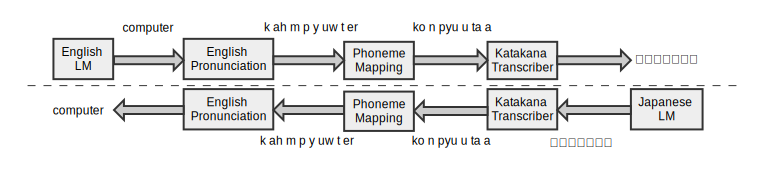
\includegraphics[scale=0.62]{figures/fsts}\tabularnewline
\end{tabular}
\caption{\label{font-table} The transliteration generative story as a cascade of FSTs . Each box represents a transducer. \textbf{Top:} transliteration of the word ``computer'' to Japanese. \textbf{Bottom:} the reverse process. PAT jointly trains the two cascades by maximizing both the data log-likelihood and the parameter agreement of the two (shaded) phoneme mapping models. The blank FSTs are held fixed. }
\label{fig:fsts}
\end{center}
\end{figure*}

Transliteration is a mapping of terms between writing systems of different languages. 
Usually, the mapping tries to preserve the sound of a term as it is uttered in the original language. 
For example, the word ``computer'' in English is transliterated to Japanese as ``ko n pyu u ta a'' (in Romaji\marginpar{Romaji or Katakana?}). 
The process restoring transliterated foreign words to their original script is called \emph{back-transliteration}.

Knight and Graehl \shortcite{KG98} suggest a generative story for the transliteration of an English term $\vw$ into Japanese term $\vk$ (see top of Figure \ref{fig:fsts}): 
\begin{enumerate}
\item First, a word $\vw$ is generated according to an English language model (LM)
$p(\vw)$.
\item $\vw$ is then mapped to an English phonemes sequence $\ve=(\ve_1,\ldots,\ve_I)$ according to a pronunciation model.
\item The phoneme sequence $\ve$ is mapped to a sequence of Japanese phonemes $\vj=(\vj_1,\ldots,\vj_J)$ according to a phoneme mapping model $p(\vj \mid \ve)$.
\item Finally, the Japanese phoneme sequence $\vj$ is mapped to a
Japanese word $\vk$ in Katakana.
\end{enumerate}
Each of their models is encoded as an FST that can be constructed and trained independently. Knight and Graehl estimate FSTs 1,2,4 over monolingual data only, whereas the phoneme mapping model $p(\vj \mid \ve)$ (\eqn{eqn:parallel}) is trained over a parallel phoneme corpus $\set{(\ve_{n},\, \vj_{n})}$ and further restricted such that each English phoneme is allowed to map to either one or two Japanese phonemes only.

However, collecting parallel data is a time consuming, laborious process.
To combat the need for parallel data, Ravi and Knight \shortcite{RK09} suggest to estimate model 2 in the decipherment setting, for which only Japanese words $K=\set{\vk_n}_{n=1}^{|K|}$ need be collected. 
Assuming one-to-one transformations for models 2 and 4 
(so that $p(\vw) = p(\ve)$ and $p(\vk) = p(\vj)$) 
the generative process for transliteration is identical to that of \eqn{eqn:decipherment}:
\begin{align*}
p(\vk)=p(\vj)
=&\sum_\vw p(\vw) \cdot p(\vj \mid \vw)\\
=&\sum_\ve p(\ve) \cdot p(\vj \mid \ve)\\
=&\sum_\ve p(\ve) \sum_\va  p(\va,  \vj \mid \ve)
\end{align*}
Where $\va=((\va_{1}^{\tstart}, \va_{1}^{\tend}),\ldots,(\va_{I}^{\tstart}, \va_{I}^{\tend}))$ denotes a \emph{source-to-target} monotone alignment sequence
under which $\ve_i$ is mapped to one or two phonemes from $\vj$, denoted $\vj[\va_{i}^{\tstart}:\va_{i}^{\tend}]$.
By monotone alignment we mean that $\va_{i}^{\cdot} \le \va_{i+1}^{\cdot}$ and $1 \le \va_{i}^{\tstart} \le \va_{i}^{\tend} \le J$ for all $i$.
The overall probability of this mapping is then:
\begin{equation}
p(\va,  \vj \mid \ve) = \prod_{i=1}^{I} t(\vj[a_{i}^{\tstart}:a_{i}^{\tend}] \mid \ve_{i})
\label{eqn:trans}
\end{equation}
where $t(\vj[a_{i}^\tstart:a_{i}^\tend] \mid \ve_{i})$ denotes the probability of transliterating English phoneme $\ve_i$ to Japanese phoneme(s) $\vj[a_{i}^\tstart:a_{i}^\tend]$.


%Thus, a Japanese phoneme sequence $\vj$ can arise from any English pronunciation sequence $\ve$ that is producible by the language and pronunciation models:
%$$
%p(\vj) = \sum_{\ve} p(\ve)\cdot p(\vj \mid \ve)$$
%As a result, the data log-likelihood takes the form:
%\begin{align}
%L(J)& = \sum_{\mathbf{j}\in J} \log \sum_{\mathbf{e}} \PP(\mathbf{j}\mid \mathbf{e})\cdot \PP(\mathbf{e})
%\end{align}
%Once the model is trained, back-transliteration (decoding) of Japanese words back to English can be done using the Viterbi algorithm.

%We note a few points:
%\begin{itemize}
%\item The computational cost of solving this problem is much higher than the parallel case since we are forced to use the language and pronunciation models during training time. 
%\item Only the phoneme mapping parameters $P(j_{m}\mid e_{m})$ are trained while
%the other FSTs' parameters are kept fixed.
%\end{itemize}









%We briefly discuss two machine translation related tasks - word alignment and phonetic back-transliteration.
%Both tasks share a similar generative story that describes how source sequences $e=(e_1, \ldots, e_I)$ (of strings or phonemes) are distorted (reordered) and translated into target sequences $f = (f_1, \ldots, e_J)$.
%As shall be seen, their sole difference lies in the permitted set of distortions - whereas all alignments are permitted in word alignment, only monotone alignments are allowed in back-transliteration.



%In machine learning, and machine translation in particular, generative stories describes transformations of entities $e$ (strings, phonemes) from a source language to entities $f$ in a target language.
%The generative story explicitly construct conditional probability distributions $P(f\mid e)$ where $e$ is an entity from $L_{E}$ and $f$ is an entity from $L_{F}$.
%The predominant approach for training generative models is the EM
%framework which iteratively maximizes log-likelihood of the observed
%data $X=\{e_{n},\, f_{n}\}_{n=1}^{N}$:
%\begin{align*}
%\max_{P}L(P\mid X)=\max_{P}\sum_{n}\log P(f_{n}\mid e_{n})
%\end{align*}
%In a setting like word alignment where models are trained in both directions, we adopt the notation $\PP(e_{n}\mid f_{n})$ for one direction and $\QQ(f_{n}\mid e_{n})$
%for the other. 
%The two models can be independently trained by maximizing each data log-likelihood function separately:
%\begin{align*}
%\PP^{*} &= \argmax_{\PP}L(\PP\mid X)\\
%\QQ^{*} &= \argmax_{\QQ}L(\QQ\mid X).
%\end{align*}
